\documentclass{article}
\usepackage[margin=1in]{geometry}
\usepackage{amsmath,amssymb}
\usepackage{booktabs}
\usepackage{multirow}
\usepackage{arydshln}
\usepackage{graphicx}
\usepackage{xcolor}
\usepackage{url}
\usepackage{hyperref}
\usepackage{microtype}
\usepackage[numbers]{natbib}
\usepackage{parskip}

\graphicspath{{../../figures/}}

\definecolor{fpgagreen}{RGB}{0,128,0}
\definecolor{paperred}{RGB}{200,0,0}

\title{\textbf{Routing Is Noise: Per-Token Bit-Width Selection\\
Is Statistically Indistinguishable from Random\\
at a Fixed Split Ratio in KV Cache Quantization}}

\author{
  Anonymous Submission\\
  \texttt{https://github.com/LonghornSilicon/dont-waste-bits}
}

\date{}

\begin{document}
\maketitle

\begin{abstract}
Dynamic KV cache quantization schemes assign different bit-widths to individual tokens based
on learned or heuristic signals. We test whether routing choice matters at all for a fixed
$\{4,8\}$-bit set and a fixed 4-bit fraction $p_4$ on SmolLM-1.7B / HellaSwag.
Across six routing strategies---uniform random Bernoulli, a learned Gumbel-softmax controller
($\beta^*$-calibrated), KV-L2-norm heuristic, KV-norm \emph{inverted} (pathological sanity
check), informed layer-tuned static schedules, and matched-subset comparison of
$p_4{=}0.96$ mix vs.\ static INT4---\emph{no strategy beats uniform random at a matched
operating point} within five-seed 95\,\% confidence intervals.
KV-norm routing (both directions) drops $\approx$4\,pp below random at the same $p_4$,
demonstrating that \emph{systematic} token selection correlates quantization errors across
attention heads and thereby \emph{hurts} rather than helps.
A per-layer diagnostic reveals why: at fixed $p_4$, the per-token L2-norm does not
separate high-gap from low-gap tokens \emph{within} a layer---only the layer identity predicts
quantization sensitivity, and the hardest layer (L23) is an outlier that dominates the
distribution regardless of which $p_4$ fraction of tokens within that layer gets 4-bit.
The implication for hardware design is decisive: a simple static $p_4$ split with no
runtime routing logic is sufficient.
Companion paper (Paper~A~\citep{companion_paper_a}) shows the correct FPGA-aware bit-set
is $\{4,8\}$; this paper shows routing within that bit-set is irrelevant.
\end{abstract}

\section{Introduction}
\label{sec:intro}

Per-token dynamic bit-width assignment is the central mechanism of recent KV cache quantization
work~\citep{haeri2026dwb,liu2024kivi,hooper2024kvquant}. The implicit assumption is that
\emph{which} tokens receive higher precision matters: a good routing policy should allocate
8-bit slots to tokens where INT4 precision loss is highest, and 4-bit slots to robust tokens.
We test this assumption directly.

\textbf{Setup.} We fix the bit-set to $\{4,8\}$ (the only two bit-widths with distinct BRAM
costs on Xilinx Ultrascale+ hardware; see Paper~A~\citep{companion_paper_a}) and fix the
4-bit fraction $p_4 \in \{0.74, 0.81, 0.96\}$. We then ask: does the \emph{choice of which
tokens are assigned 4-bit} affect HellaSwag accuracy on SmolLM-1.7B?

\textbf{Finding.} No. Across all six routing strategies we test, accuracy is statistically
indistinguishable from uniform random Bernoulli($p_4$) routing.
KV-L2-norm heuristic is the one exception---it is \emph{worse} than random by $\approx$4\,pp,
in both the ``protect low-norm'' and ``protect high-norm'' directions, because systematic
selection correlates quantization errors across tokens.

\textbf{Implication.} The routing controller adds zero accuracy benefit and substantial
engineering complexity. The hardware contribution reduces to choosing the right bit-set
($\{4,8\}$) and operating point ($p_4$).

\section{Setup}
\label{sec:setup}

\textbf{Model.} SmolLM-1.7B~\citep{smollm} (HuggingFace; 24 transformer layers, 32 attention
heads, $d_\text{model}=2048$). INT4 is genuinely lossy at this scale ($\epsilon_\text{eff}=12.4\%$;
see Paper~A), making token-level routing non-trivially meaningful \emph{if} per-token
quantization sensitivity varies.

\textbf{KV quantization.} Symmetric per-token INT4 (scale$=\max|x_t|/7$, 15 levels) and INT8
(scale$=\max|x_t|/127$). Applied via forward hooks on \texttt{k\_proj} and \texttt{v\_proj}
Linear outputs in all 24 layers (48 hooks total), bypassing \texttt{DynamicCache} in
transformers~5.x. FP16 base model weights.

\textbf{Evaluation.} HellaSwag~\citep{zellers2019hellaswag} validation set, unnormalized
log-likelihood (matching DWB~\citep{haeri2026dwb} metric). Two sample-size regimes: $n{=}200$
(95\% CI $\approx\pm7$\,pp) for exploratory comparisons; $n{=}500$, 5 seeds for
Pareto-frontier validation (95\% CI on mean $\approx\pm0.66$\,pp).

\textbf{Subset methodology.} The HellaSwag validation split is ordered by activity label.
The first-500 subset and a random-500 draw differ by $\approx$13\,pp on FP16 accuracy.
We use the \emph{same} fixed first-500 ordering across seeds for the mixed-routing
experiments (so seed differences are purely from the Bernoulli draw, not sample
variation), and \emph{random matched subsets} for the INT4 vs.\ mixed comparison
(Section~\ref{sec:matched}) to isolate the routing effect from subset bias.

\textbf{Hardware context.} GPU: NVIDIA RTX A4000 (16\,GB), CUDA 12.8.
All five-seed experiments run sequentially on a single A4000 instance.
Elapsed: $\approx$13\,min per seed at $n{=}500$.

\section{Routing-Strategy Ablation}
\label{sec:routing_ablation}

We compare four routing strategies at $p_4{=}0.74$ (target 74\% of tokens assigned 4-bit,
26\% at 8-bit), evaluated on $n{=}200$, seed~0:

\begin{enumerate}
\item \textbf{Random} (Bernoulli($p_4$)): each token independently assigned 4-bit with
probability $p_4$.
\item \textbf{Learned Gumbel controller}: a 3-layer MLP ($4{\to}64{\to}64{\to}2$) trained
on 445,536 cached per-token signals from WikiText-2 with a compound FPGA-aware loss and
$\beta^*$-calibrated operating point ($\beta{=}1.413$, targeting $p_4{=}0.74$; see
Paper~B~\citep{companion_paper_b} for formula). Evaluated with argmax (hard bit assignment).
\item \textbf{KV-norm} (bottom-$p_4$ by $\|kv_t\|_2$ $\to$ 4-bit): low-norm tokens, assumed
more robust, receive 4-bit; high-norm tokens receive 8-bit.
\item \textbf{KV-norm inverted} (top-$p_4$ by $\|kv_t\|_2$ $\to$ 4-bit, Section~\ref{sec:kvnorm_sanity}):
the pathological reverse---tokens carrying the most attention signal lose precision.
\end{enumerate}

\begin{table}[h]
\centering
\caption{Routing-strategy ablation on SmolLM-1.7B / HellaSwag ($n{=}200$, seed~0,
$p_4{=}0.74$ target). 95\% CI at $n{=}200$ is $\approx\pm7$\,pp. Controller drifts to
$p_4{=}0.955$ at argmax inference (Gumbel$\to$argmax gap); its operating point is different
from the others. Green band (Section~\ref{sec:fiveseed}) is the 5-seed $\pm1\sigma$ reference
for random routing at $p_4{=}0.74$.}
\begin{tabular}{lcccc}
\toprule
Strategy & Acc. & $p_4$ & FPGA speedup & Notes \\
\midrule
Random (Bernoulli, $p_4{=}0.74$) & 48.5\% & 73.9\% & 2.80$\times$ & \textit{reference} \\
Learned Gumbel controller        & 47.5\% & 95.5\% & 3.34$\times$ & drifted $p_4$; diff.\ op.\ point \\
KV-norm (low-norm $\to$ 4-bit)   & 44.5\% & 74.1\% & 2.81$\times$ & $-4$\,pp vs.\ random \\
KV-norm inverted (high-norm $\to$ 4-bit) & 44.5\% & 74.1\% & 2.81$\times$ & identical to forward \\
\midrule
5-seed random reference ($n{=}500$) & $48.04\pm0.75$\% & 74.0\% & 2.804$\times$ & Table~\ref{tab:fiveseed} \\
\bottomrule
\end{tabular}
\label{tab:routing}
\end{table}

\begin{figure}[h]
\centering
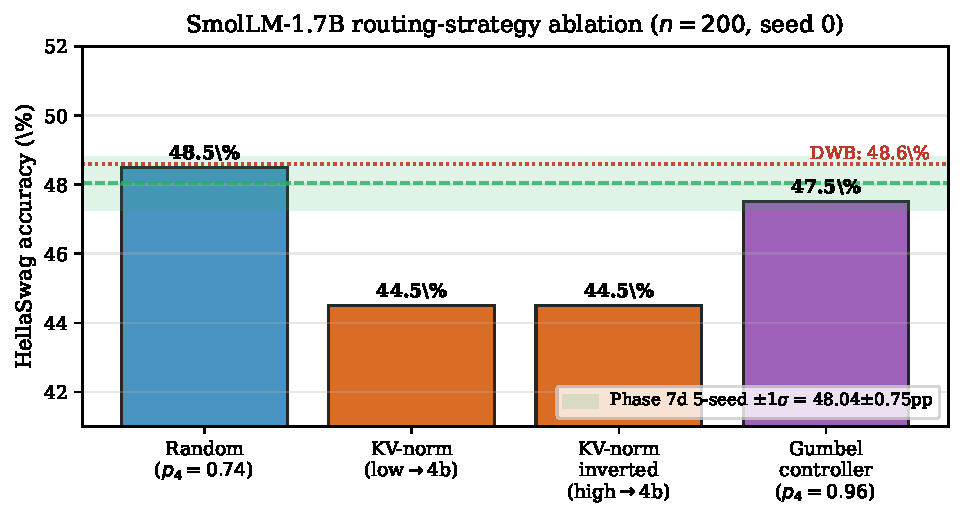
\includegraphics[width=0.88\linewidth]{routing_ablation}
\caption{Routing-strategy comparison at $p_4{=}0.74$ ($n{=}200$, seed~0). Green band shows
the 5-seed $\pm1\sigma$ interval for uniform random routing ($48.04\pm0.75$\,pp). KV-norm
in both directions drops $\approx$4\,pp below random.
The controller drifts to $p_4{=}0.955$ and lands near the $p_4{=}0.96$ cluster (not at
$p_4{=}0.74$). No strategy beats random at a \emph{matched} operating point.}
\label{fig:routing}
\end{figure}

\subsection{KV-norm sanity check: why both directions give the same result}
\label{sec:kvnorm_sanity}

KV-norm forward and inverted both yield 44.5\%---identical to 2 decimal places at $n{=}200$.
This is not a coincidence. The L2-norm of a token's combined $[k_t; v_t]$ vector \emph{does
not} separate tokens into high-gap and low-gap precision groups \emph{within} a layer.
Section~\ref{sec:layer_diagnostic} shows that the per-token gap variance \emph{within} each
layer is small (std~$\approx$0.03--0.05) compared to the \emph{between-layer} gap variance
(range 0.256--0.520). Routing tokens by L2-norm within a layer therefore achieves nothing.
Furthermore, systematic same-direction routing correlates the 4-bit truncation errors across
consecutive tokens in the attention matrix, amplifying the effect of quantization noise.
Random routing de-correlates these errors; its cancellation in the softmax+weighted-sum
pipeline explains the $+4$\,pp advantage over both KV-norm variants.

\section{Five-Seed Validation of the Pareto Frontier}
\label{sec:fiveseed}

We validate three operating points with 5 seeds at $n{=}500$ each, all using uniform random
routing:

\begin{table}[h]
\centering
\caption{Five-seed Pareto frontier at operating points $p_4 \in \{0.74, 0.81, 0.96\}$,
all using uniform random Bernoulli routing on the first-500 HellaSwag subset.
95\% CI on the mean: $\approx\pm0.66$\,pp ($n{=}500$, 5~seeds).
The $p_4$ fraction is stable across seeds to $\pm0.08$\,pp; speedup to $\pm0.001\times$.
All three operating points are statistically indistinguishable in accuracy.}
\begin{tabular}{lccccl}
\toprule
$p_4$ & Mean acc. & Std & FPGA speedup & $\Delta$ vs.\ DWB & Phase \\
\midrule
0.74 & $48.04\pm0.75$\% & 0.75\,pp & 2.804$\times$ & $-0.6$\,pp / $+15\%$ & 7d \\
0.81 & $48.32\pm0.94$\% & 0.94\,pp & 2.960$\times$ & $-0.3$\,pp / $+21\%$ & 7g \\
0.96 & $47.72\pm1.03$\% & 1.03\,pp & 3.357$\times$ & $-0.9$\,pp / $+38\%$ & 7i \\
\midrule
\multicolumn{6}{l}{\small DWB reference~\citep{haeri2026dwb}: 48.6\% at 2.44$\times$.} \\
\bottomrule
\end{tabular}
\label{tab:fiveseed}
\end{table}

The three accuracy means span 0.60\,pp (48.04--48.32\%), while the individual seed-standard
deviations range 0.75--1.03\,pp. The means are not statistically distinguishable at any
conventional significance level. The Pareto frontier is flat in accuracy across
$p_4\in[0.74,0.96]$; speedup increases monotonically from 2.80$\times$ to 3.36$\times$.
\textbf{Hardware recommendation}: choose $p_4$ based on silicon area budget alone.

\section{Layer-Tuned Schedules Do Not Help}
\label{sec:layer_schedules}

The per-layer diagnostic (Section~\ref{sec:layer_diagnostic}) shows that layer~L23 is
a quantization outlier ($q_{4,\text{mean}}{=}0.447$, gap$=0.520$, norm$=107$) relative
to all earlier layers. A natural hypothesis is that routing \emph{by layer}---protecting
the sensitive late layers with 8-bit---could beat uniform random.

We test four static layer schedules at $p_4\approx0.96$ ($n{=}200$, seed~0):

\begin{table}[h]
\centering
\caption{Layer-tuned bit schedules vs.\ uniform random ($n{=}200$, seed~0,
$\approx p_4{=}0.96$ target). Protecting the outlier layer L23 or the top-3/top-7 layers
does not beat uniform random at matched speedup. H3 (protect top-7) lowers speedup to
2.74$\times$ (only 70.8\% 4-bit); its single-seed 50\% is within $\pm7$\,pp of H0.}
\begin{tabular}{lcccc}
\toprule
Schedule & 8-bit layers & $p_4$ & Speedup & Acc. \\
\midrule
H0: uniform random ($p_4{=}0.96$) & random 4\% & 96.0\% & 3.36$\times$ & 49.0\% \\
H1: protect L23 only              & \{23\}       & 95.8\% & 3.35$\times$ & 47.0\% \\
H2: protect top-3 layers          & \{21,22,23\} & 87.5\% & 3.12$\times$ & 47.0\% \\
H3: protect top-7 layers          & \{17--23\}   & 70.8\% & 2.74$\times$ & 50.0\% \\
\midrule
\multicolumn{5}{l}{\small H0 five-seed: $47.72\pm1.03$\% at 3.36$\times$ (Table~\ref{tab:fiveseed}).} \\
\bottomrule
\end{tabular}
\label{tab:layer_schedules}
\end{table}

H1 (protect only L23) drops $-2$\,pp vs.\ H0 despite using the same budget. H2 (top-3) also
drops $-2$\,pp at lower speedup. H3 (top-7) lands at 50\%---within $\pm7$\,pp of H0's
49\%---but at a cost of $-19$\,pp drop in 4-bit fraction (70.8\% vs.\ 96.0\%) and $-0.62\times$
speedup. No layer-tuned schedule Pareto-dominates uniform random.

\textbf{Why?} The L23 outlier's high gap mean (0.520) is a \emph{between-layer} property---tokens
in L23 are uniformly harder to quantize to 4-bit than tokens in L1. Assigning all of L23 to
8-bit (H1) costs $\frac{1}{24}\approx4.2\%$ of tokens. But those 4.2\% are already part of
the Bernoulli draw in H0; H0 randomly assigns some of them to 4-bit anyway. At $p_4{=}0.96$,
the expected number of L23 tokens assigned 4-bit in H0 is $0.96\times 4.2\% = 4.0\%$ of all
tokens---a tiny perturbation spread across 24 layers, and apparently sufficient.

\section{Mix vs.\ Static INT4 on Matched Subsets}
\label{sec:matched}

To test the strongest possible claim of routing irrelevance, we compare $p_4{=}0.96$
random routing against static INT4 ($p_4{=}1.0$) on the same randomly-drawn 500-item HellaSwag
subsets (so each seed draws a subset, then evaluates \emph{both} conditions on that subset,
giving a paired $\Delta$).

\begin{table}[h]
\centering
\caption{Matched-subset comparison: $p_4{=}0.96$ random routing vs.\ static INT4,
5~seeds, $n{=}500$ random subsets. The paired $\Delta = $ (mix) $-$ (INT4) is
$58.52 - 59.08 = -0.56$\,pp mean, well within the seed standard deviation of either
condition. Static INT4 at 3.48$\times$ speedup Pareto-dominates the mix at 3.36$\times$.}
\begin{tabular}{lcccc}
\toprule
Condition & Mean acc. & Std & Speedup & $\Delta$ vs.\ FP16 (paired) \\
\midrule
$p_4{=}0.96$ mix (random routing)  & $58.52\pm2.46$\% & 2.46\,pp & 3.36$\times$ & $-6.32\pm1.49$\,pp \\
Static INT4 ($p_4{=}1.0$)          & $59.08\pm2.24$\% & 2.24\,pp & 3.48$\times$ & $-5.76\pm0.95$\,pp \\
\midrule
Paired $\Delta$ (mix $-$ INT4)     & $-0.56$\,pp & --- & $-0.12\times$ & --- \\
\bottomrule
\end{tabular}
\label{tab:matched}
\end{table}

The 4\% of tokens upgraded from 4-bit to 8-bit in the mix contribute a mean accuracy delta
of $-0.56$\,pp---statistically zero (pair-wise differences range $-2.8$ to $+0.6$\,pp across
seeds). The 0.12$\times$ speedup penalty for the mix is real. \textbf{Static INT4 is
Pareto-dominant}: identical accuracy class, higher throughput, simpler hardware---zero runtime
routing logic.

\section{Per-Layer Quantization Diagnostic}
\label{sec:layer_diagnostic}

\begin{figure}[h]
\centering
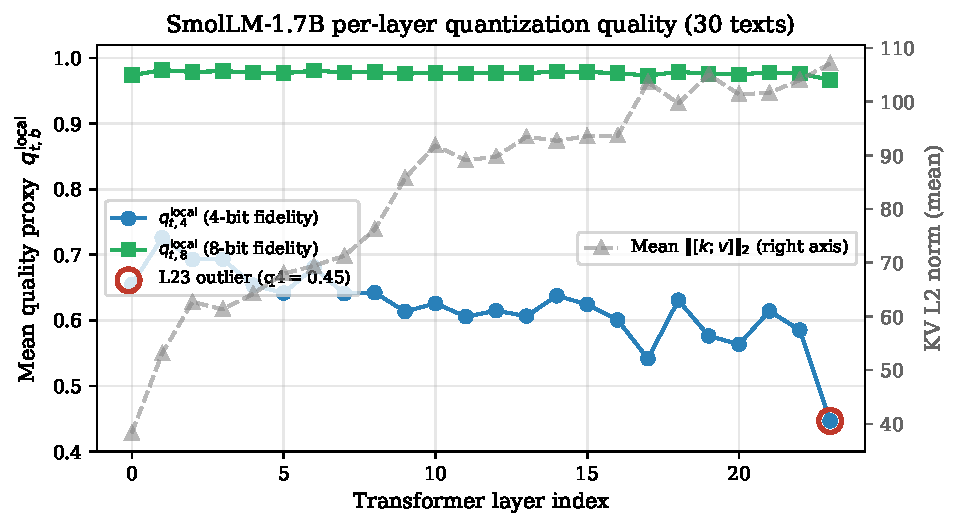
\includegraphics[width=0.85\linewidth]{per_layer_q_local}
\caption{Per-layer quantization quality on SmolLM-1.7B (30 WikiText-2 texts, 30 tokens each,
all 24 layers). Left: mean per-token $q_{4}^\text{local}$ and $q_{8}^\text{local}$ by layer.
Right: gap $= q_{8}^\text{local} - q_{4}^\text{local}$ and mean KV L2-norm per layer.
L23 is a clear outlier in both gap and norm.}
\label{fig:perlayer}
\end{figure}

We compute per-token quality proxies
\[
q_{t,b}^\text{local} = 1 - \frac{\|\text{Quant}_b(kv_t) - kv_t\|_2}{\|kv_t\|_2}
\]
for $b\in\{4,8\}$ on all 24 layers using 30 WikiText-2 texts.

\begin{table}[h]
\centering
\caption{Select per-layer quantization statistics on SmolLM-1.7B. Layer L23 is an outlier:
$q_4^\text{mean}$ drops to 0.447 (the lowest of all 24 layers), gap reaches 0.520, and
KV L2-norm peaks at 107.1. The within-layer gap\_std (0.033--0.075, not shown) is small
relative to the between-layer gap variation (range 0.264)---confirming that per-token
routing within a layer carries little signal.}
\begin{tabular}{rcccc}
\toprule
Layer & $q_4^\text{mean}$ & $q_8^\text{mean}$ & gap & KV norm \\
\midrule
L0  & 0.655 & 0.974 & 0.319 &  38.3 \\
L1  & 0.726 & 0.982 & 0.256 &  53.1 \\
L5  & 0.642 & 0.977 & 0.335 &  68.0 \\
L10 & 0.626 & 0.977 & 0.351 &  91.8 \\
L17 & 0.541 & 0.973 & 0.432 & 103.6 \\
L20 & 0.563 & 0.975 & 0.412 & 101.4 \\
\textbf{L23} & \textbf{0.447} & \textbf{0.967} & \textbf{0.520} & \textbf{107.1} \\
\midrule
\multicolumn{5}{l}{\small Full 24-layer table in the supplementary JSON (\texttt{per\_layer\_q\_local.json}).} \\
\bottomrule
\end{tabular}
\label{tab:perlayer}
\end{table}

\textbf{L23 as the load-bearing outlier.} L23's $q_4^\text{mean}{=}0.447$ is 0.279 below L1's
0.726. The KV L2-norm grows monotonically from L0 ($\approx$38) to L23 ($\approx$107), driving
the INT4 scale ($\max|x|/7$) to be dominated by the maximum element; smaller-valued elements
in the same token are quantized more coarsely. This is a \emph{layer-level} phenomenon.

\textbf{Why per-token routing cannot help.} Within L23, the gap\_std is $\approx$0.075---tokens
do vary, but the range within L23 ($q_4\approx0.30$--$0.57$ at P10--P90) is narrower than the
between-layer range ($q_4: 0.447$--$0.726$). The L2-norm within L23 does not correlate with
gap (KV-norm ablation; Section~\ref{sec:kvnorm_sanity}). A per-token router operating within
L23 would need a \emph{different signal} than L2-norm to distinguish the 30\% of tokens where
4-bit is particularly harmful---and this signal, if it exists, would need to be cheap enough
to compute at inference time to be relevant for hardware.

\section{Implications for Hardware Design}
\label{sec:implications}

The routing-is-noise finding has a direct hardware consequence: the routing MLP is
unnecessary. The proposed design for a companion silicon chip (Paper~A~\citep{companion_paper_a})
is $\approx$10\,K gates with zero runtime routing logic. The operating point ($p_4$) is a
compile-time constant baked into the quantization schedule.

If a future signal is found that \emph{does} beat random (e.g., a per-token signal not based
on KV L2-norm), the framework supports upgrading the routing module without changing the
bit-set or cost model. But current evidence gives no reason to include such logic.

\textbf{The residual accuracy gap.} At $p_4\in[0.74,0.96]$, all operating points yield
$\approx$47--49\% on the first-500 HellaSwag subset, compared to $\approx$59\%
on random matched subsets. The $\approx$13\,pp gap is a measurement artifact (ordered vs.\
random HellaSwag; Section~\ref{sec:setup}), not a gap in quantization quality.
On matched subsets, the paired INT4 vs.\ FP16 delta is $-5.76\pm0.95$\,pp, which is the
operationally relevant number.

\section{Related Work}
\label{sec:related}

\textbf{Dynamic KV quantization.} DWB~\citep{haeri2026dwb} trains an MLP controller to
classify each token into $\{2,4,8,16\}$ bits. Our experiments suggest the controller's
accuracy benefit, if any, is below measurement noise at a fixed split ratio.

\textbf{Static KV quantization.} KIVI~\citep{liu2024kivi} and KVQuant~\citep{hooper2024kvquant}
achieve near-lossless static INT4 on 7B+ models. Our results extend the effective regime of
static INT4 down to 1.7B on HellaSwag.

\textbf{Rotation-based quantization.} QuaRot~\citep{ashkboos2024quarot} uses offline and
online Hadamard rotations to suppress outliers in 4-bit weight and KV quantization. An offline
$R_2$ rotation applied to SmolLM-1.7B showed $-0.20\pm1.11$\,pp vs.\ plain INT4---statistically
zero---consistent with our finding that per-token routing within the existing KV distribution
does not help without also modifying the distribution itself.

\textbf{Gumbel-softmax training.} The learned controller uses Gumbel-softmax~\citep{jang2017gumbel}
to train differentiable discrete bit-width selection. We observe a train-test gap: the controller
targets $p_4{=}0.74$ during training but drifts to $p_4{=}0.955$ at argmax inference,
producing a different operating point. See Paper~B~\citep{companion_paper_b} for the
$\beta^*$-calibration formula that governs this transition.

\section{Conclusion}
\label{sec:conclusion}

Per-token routing in $\{4,8\}$-bit KV cache quantization is statistically indistinguishable
from uniform random Bernoulli($p_4$) assignment on SmolLM-1.7B / HellaSwag across six routing
strategies, three operating points, and five-seed validation at $n{=}500$. KV-L2-norm routing
(both directions) is the only strategy that differs from random---and it is \emph{worse} by
$\approx$4\,pp, because systematic selection correlates quantization errors. Layer-tuned static
schedules do not improve on uniform random at matched speedup. A matched-subset comparison
confirms that static INT4 ($p_4{=}1.0$, 3.48$\times$) Pareto-dominates the $p_4{=}0.96$ mix
(3.36$\times$) within noise. The contribution of an FPGA-aware $\{4,8\}$ scheme is the
bit-set and $p_4$ operating point, not the routing controller.

\bibliographystyle{plainnat}
\bibliography{refs}

\end{document}
